\section{Event Transmission}

The event transmitter is somewhat complex due to the desire to avoid
sending packets with no / few events, but to also avoid event
overflow. A worst-case would be every single event in an event cycle
being directed at the network device; This would result in 960 bytes
of data for the UDP packet. But sending a single event wastes 80% of
the ethernet frame capacity. But we also wish to avoid prolonged
periods of event queuing, which hurts latency. 

To meet these parameters, we send an event datagram whenever: 
\begin{enumerate}
\item More than 5 ecycles have passed without a transmission
\item There is not enough empty space in the current packet to send the current ecycle. 
\end{enumerate} 

Each event cycle's events are termed an ``Event Set''; an Event Set is
written into the transmitted UDP packet with an EVTLEN header
indicating the number of events in the Set. Up to five event sets are
included in an event packet.

\subsection{Implementation}
\begin{figure}
\begin{centering}
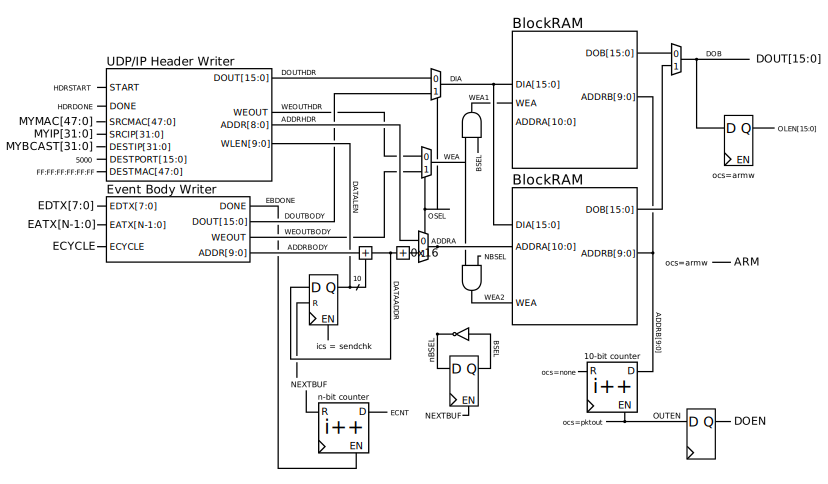
\includegraphics[scale=0.8]{eventtx.svg}
\end{centering}
\caption{Event transmission implementation}
\label{eventtx}
\end{figure}

\begin{figure}
\begin{centering}
\includegraphics[scale=0.8]{eventtx.fsm.svg}
\end{centering}
\caption{Event transmission implementation FSM.}
\label{eventtx.fsm}
\end{figure}

At 50 MHz, a 1024-byte event takes 10.3 $\mu s$ to transmit. We need to
maintain the ability for the network TX interface to transmit one of
these per cycle.

Our implementation uses separate modules to write the relevant bits for
the IP/UDP headers and the data. 

Each module writes into an EventTx Packet FIFO, which is a 4-deep fifo
with the relevant bits of an event UDP datagram as constants (such as
protocol number). We use two of these FIFOs, one for eventual output
to the network interface, and one for output to the retransmission
buffer. The two distinct outputs allow for the different interfaces to
receive data at different rates.

Note our interface depends quite heavily on the implicit timing from
the event bus. In particular, upon assertion of an ECYCLE, we wait ~5
ticks until we have counted the number of events in this cycle. Then,
if this will ``break the bank'' we must commit the current buffer
\textit{and} reset all relevant logic before the Event Body Writer
begins writing the current event's packets.

We use the standard UDP/IP header Writer to write the packet header data. 

\subsection{Event Body Writer}
\begin{figure}
\begin{centering}
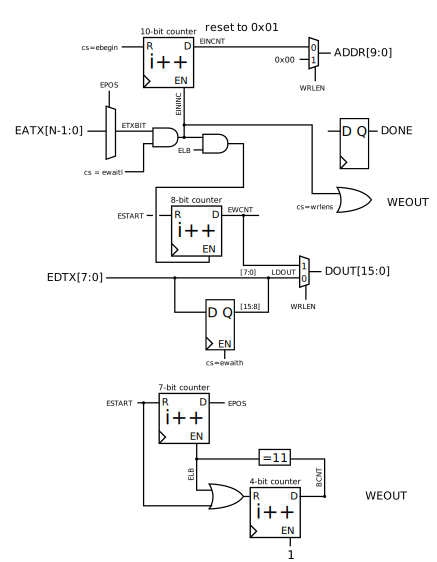
\includegraphics[scale=0.8]{eventtx.eventbody.svg}
\end{centering}
\caption{Event transmission event body writer}
\label{eventtx.eventbody}
\end{figure}

\begin{figure}
\begin{centering}
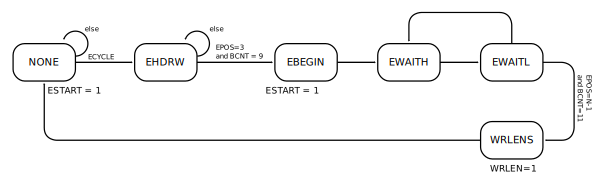
\includegraphics[scale=0.8]{eventtx.eventbody.fsm.svg}
\end{centering}
\caption{Event transmission event body writer}
\label{eventtx.eventbody.fsm}
\end{figure}

The eventbodywriter receives events via an Event Port and writes an entire event set into the output packet FIFO. It does this by: 

\begin{enumerate}
\item Writes the event data bytes, aggregating them into 16-bit words, out \signal{DOUT[15:0]} with the assertion of \signal{WEOUT}. 
\item After the event words are written, writes the number-of-events-written to byte 0
\item then asserts done. 
\end{enumerate}

We are guaranteed at least 40 ticks between the assertion of ECYCLE
and the first assertion of WEOUT for that cycle. 

At the assertion of DONE, we verify/guarantee that ADDR contains the
address of the word that is one-past the last written word. For
example, if we wrote one event, then the len was written at addr 0,
the event was in 1-12, and ADDR will equal 13 when DONE is asserted,
and stay at that for 40 ticks.


\subsection{EventTX Packet FIFO}
\begin{figure}
\begin{centering}
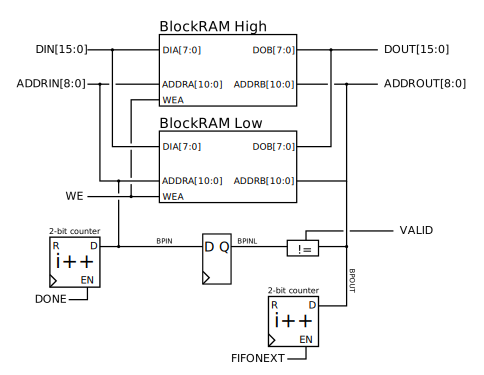
\includegraphics[scale=0.8]{eventtx.packetfifo.svg}
\end{centering}
\caption{The Event Packet TX FIFO is a simple 4-packet-deep .} 
\label{eventpktfifo}
\end{figure}

The EventTX Packet FIFO stores up to four packets to account for
timing differences between timing of input and output. 


\subsection{Bit Counter}
The Bit Counter (figure \ref{bitcounter}) is used to efficiently count
the number of bits set in an event address word. \signal{START} is
asserted with an event address array presented at \signal{DIN[95:0]}.
Four cycles later \signal{DONE} is asserted signalling completion with
the number of set bits available at \signal{DOUT[6:0]}.


\begin{figure}
\begin{centering}
\includegraphics[scale=0.8]{bitcnt.svg}
\end{centering}
\caption{BitCounter is used to efficiently count the number of bits set in an event address mask.}
\label{bitcounter}
\end{figure}

